\chapter{RELEASE 1}
\addcontentsline{toc}{chapter}{Chapitre 3 : RELEASE 1}

\section*{Introduction}
\addcontentsline{toc}{section}{Introduction}
Après avoir exposé en détail les exigences de notre projet à travers un backlog produit, nous entamons dans ce chapitre la première version du projet, qui comprend deux sprints : le sprint 1 et le sprint 2. Chaque sprint couvre l'analyse, la conception et la réalisation.

\section{Organisation du sprint}
Notre release est composée de deux sprints :\\
\textbf{- Sprint 1 :} Configuration initiale et base du projet.\\
\textbf{- Sprint 2 :} Authentification et gestion des utilisateurs.

\section{Sprint 1 : Configuration initiale et base du projet}
\subsection{Objectif du sprint}
L'objectif de ce sprint est de mettre en place l'environnement MERN, la configuration backend et frontend. Les tâches principales sont :
\begin{itemize}
    \item l'initialisation du dépôt Git ;
    \item la création du serveur Express avec une route de test ;
    \item la modélisation de la base de données MongoDB ;
    \item la configuration de React.js et des routes principales.
\end{itemize}

\section{Sprint 2 : Authentification et gestion des utilisateurs}
\subsection{Objectif du sprint}
L'objectif de ce sprint est de mettre en place un système d'authentification (JWT) et une gestion des rôles. Les tâches principales sont :
\begin{itemize}
    \item la création des modèles utilisateurs avec rôles ;
    \item l'implémentation des routes d'authentification et la gestion des sessions avec JWT ;
    \item l'interface React pour l'inscription et la connexion.
\end{itemize}

\subsection{Sprint backlog}
Le deuxième sprint s'étend du 12 février au 21 février. Le tableau suivant représente le backlog de ce sprint.

\renewcommand{\arraystretch}{1.6}
\setlength{\tabcolsep}{5pt}
\begin{longtable}{|c|c|m{7cm}|c|c|}
\caption{User Stories – Sprint Authentification et gestion des utilisateurs} \\
\hline
\textbf{ID} & \textbf{Sprint} & \textbf{User Story} & \textbf{Priorité} & \textbf{Complexité} \\
\hline
\endfirsthead

\hline
\textbf{ID} & \textbf{Sprint} & \textbf{User Story} & \textbf{Priorité} & \textbf{Complexité} \\
\hline
\endhead

\hline
\endfoot

\hline
\endlastfoot

2 & \parbox{3cm}{\centering Authentification et\\ gestion des utilisateurs} 
& En tant qu'utilisateur, je souhaite créer un compte. & Élevée & Moyenne \\
\hline
2 & \parbox{3cm}{\centering Authentification et\\ gestion des utilisateurs} 
& En tant qu'utilisateur, je souhaite m'authentifier. & Élevée & Moyenne \\
\hline
2 & \parbox{3cm}{\centering Authentification et\\ gestion des utilisateurs} 
& En tant que gestionnaire, je souhaite créer un compte. & Élevée & Moyenne \\
\hline
2 & \parbox{3cm}{\centering Authentification et\\ gestion des utilisateurs} 
& En tant que gestionnaire, je souhaite m'authentifier. & Élevée & Moyenne \\
\hline
2 & \parbox{3cm}{\centering Authentification et\\ gestion des utilisateurs} 
& En tant qu'administrateur, je veux créer un utilisateur pour la gestion des utilisateurs. & Élevée & Moyenne \\
\hline
2 & \parbox{3cm}{\centering Authentification et\\ gestion des utilisateurs} 
& En tant qu'administrateur, je veux modifier un utilisateur pour la gestion des utilisateurs. & Élevée & Moyenne \\
\hline
2 & \parbox{3cm}{\centering Authentification et\\ gestion des utilisateurs} 
& En tant qu'administrateur, je veux supprimer un utilisateur pour la gestion des utilisateurs. & Élevée & Moyenne \\
\hline
2 & \parbox{3cm}{\centering Authentification et\\ gestion des utilisateurs} 
& En tant qu'administrateur, je veux consulter un utilisateur pour la gestion des utilisateurs. & Élevée & Moyenne \\
\hline
\end{longtable}

\subsection{Implémentation du sprint 2}
\subsubsection{Spécification des besoins}
Dans cette section, nous identifions les besoins de notre deuxième sprint, à travers :
\begin{itemize}
    \item les diagrammes de cas d'utilisation,
    \item les descriptions textuelles associées,
    \item les diagrammes de séquences système.
\end{itemize}

\textbf{La figure ci-dessous représente le premier diagramme de cas d'utilisation de ce sprint.}

\begin{figure}[H]
    \centering
    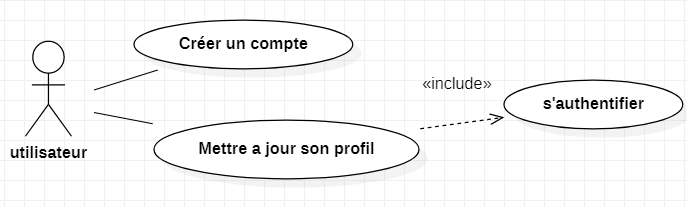
\includegraphics[width=0.6\linewidth]{projet/images/diagramme de sequance/images/utilisateur.png}
    \caption{Diagramme des cas d'utilisation « S'authentifier (Utilisateur) »}
    \label{fig:equipe_scrum}
\end{figure}

Ce diagramme décrit le processus d'authentification de l'utilisateur. Nous détaillons ci-après ce cas d'utilisation sous forme textuelle :

\begin{longtable}{|>{\bfseries}p{4cm}|p{10cm}|}
\hline
Cas d'utilisation & S'inscrire \\
\hline
Acteurs & Utilisateur \\
\hline
Précondition & L'utilisateur demande l'interface d'inscription \\
\hline
Post-condition & Le compte est créé \\
\hline
Scénario principal & 
\begin{enumerate}
  \item Le système affiche la page d'inscription de connexion
  \item L'utilisateur remplit le formulaire et le soumet
  \item Le système vérifie les informations et crée le compte
  \item Le système affiche un message de succès
\end{enumerate} \\
\hline
Scénario alternatif & Le système affiche un message d'erreur si le login ou mot de passe sont incorrects \\
\hline
\caption{Description textuelle du cas d'utilisation pour Créer un compte}
\end{longtable}

\begin{longtable}{|>{\bfseries}p{4cm}|p{10cm}|}
\hline
Cas d'utilisation & S'authentifier (Utilisateur) \\
\hline
Acteurs & Utilisateur \\
\hline
Précondition & L'utilisateur possède un login et un mot de passe \\
\hline
Post-condition & Utilisateur Authentifié \\
\hline
Scénario principal & 
\begin{enumerate}
  \item Le système affiche l'interface qui contient un formulaire de connexion
  \item L'utilisateur saisit son login et son mot de passe
  \item Il confirme en cliquant sur le bouton « se connecter »
  \item Le système affiche l'interface d'accueil propre à l'utilisateur
\end{enumerate} \\
\hline
Scénario alternatif & Le système affiche un message d'erreur si le login ou mot de passe sont incorrects \\
\hline
\caption{Description textuelle du cas d'utilisation « S'authentifier (Utilisateur) »}
\end{longtable}

\textbf{La figure ci-dessous représente le deuxième diagramme de cas d'utilisation de ce sprint.}

\begin{figure}[H]
    \centering
    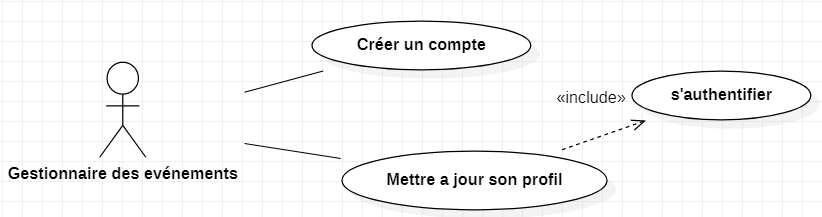
\includegraphics[width=0.6\linewidth]{projet/images/diagramme de sequance/images/gestionnaire.png}
    \caption{Diagramme des cas d'utilisation « S'authentifier (Gestionnaire) »}
    \label{fig:equipe_scrum}
\end{figure}

Ce diagramme décrit le processus d'authentification de gestionnaire. Nous détaillons ci-après ce cas d'utilisation sous forme textuelle :

\begin{longtable}{|>{\bfseries}p{4cm}|p{10cm}|}
\hline
Cas d'utilisation & S'inscrire \\
\hline
Acteurs & Gestionnaire \\
\hline
Précondition & Gestionnaire demande l'interface d'inscription \\
\hline
Post-condition & Le compte est créé \\
\hline
Scénario principal & 
\begin{enumerate}
  \item Le système affiche la page d'inscription de connexion
  \item Gestionnaire remplit le formulaire et le soumet
  \item Le système vérifie les informations et crée le compte
  \item Le système affiche un message de succès
\end{enumerate} \\
\hline
Scénario alternatif & Le système affiche un message d'erreur si le login ou mot de passe sont incorrects \\
\hline
\caption{Description textuelle du cas d'utilisation pour Créer un compte}
\end{longtable}

\begin{longtable}{|>{\bfseries}p{4cm}|p{10cm}|}
\hline
Cas d'utilisation & S'authentifier (gestionnaire) \\
\hline
Acteurs & Gestionnaire \\
\hline
Précondition & L'utilisateur possède un login et un mot de passe \\
\hline
Post-condition & Utilisateur Authentifié \\
\hline
Scénario principal & 
\begin{enumerate}
  \item Le système affiche l'interface qui contient un formulaire de connexion
  \item L'utilisateur saisit son login et son mot de passe
  \item Il confirme en cliquant sur le bouton « se connecter »
  \item Le système affiche l'interface d'accueil propre de gestionnaire
\end{enumerate} \\
\hline
Scénario alternatif & Le système affiche un message d'erreur si le login ou mot de passe sont incorrects \\
\hline
\caption{Description textuelle du cas d'utilisation « S'authentifier (Gestionnaire) »}
\end{longtable}

\textbf{La figure ci-dessous représente le troisième diagramme de cas d'utilisation de ce sprint.}

\begin{figure}[H]
    \centering
    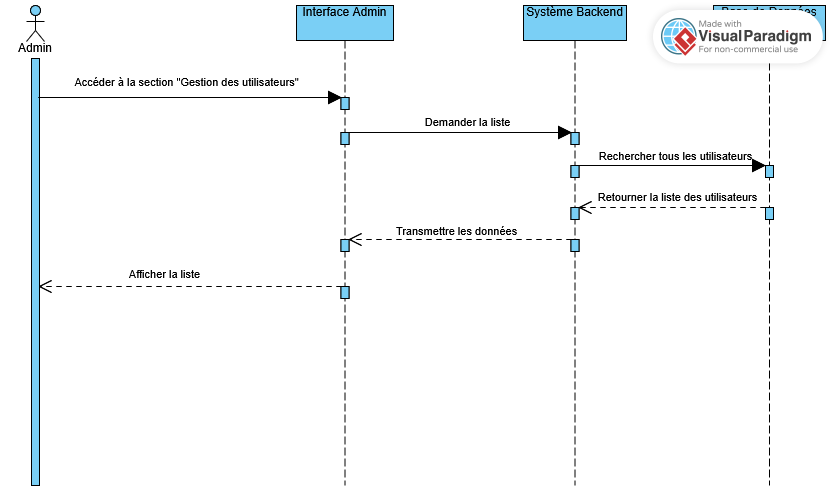
\includegraphics[width=0.6\linewidth]{projet/images/diagramme de sequance/consulter les utilisateurs admin sequnace diagram(1).png}
    \caption{Diagramme des cas d'utilisation « gestion d'utilisation »}
    \label{fig:equipe_scrum}
\end{figure}

Ce diagramme de cas d'utilisation représente le processus de gestion d'utilisateur, qui se manifeste dans l'ajout, la modification, la suppression, la consultation de la liste d'utilisateur. Nous détaillons ci-après ce cas d'utilisation sous forme textuelle :

\begin{longtable}{|>{\bfseries}p{4cm}|p{10cm}|}
\hline
Cas d'utilisation & Créer un utilisateur \\
\hline
Acteurs & Administrateur \\
\hline
Précondition & Authentification préalable \\
\hline
Post-condition & Utilisateur est ajouté \\
\hline
Scénario principal & 
\begin{enumerate}
  \item L'administrateur clique sur le bouton d'ajout d'un utilisateur
  \item Le système affiche le formulaire d'ajout d'un utilisateur
  \item L'administrateur remplit le formulaire avec les informations du l'utilisateur et le soumet
  \item Le système vérifie les informations et ajoute l'utilisateur
  \item Le système affiche un message de succès
\end{enumerate} \\
\hline
Scénario alternatif & 
\begin{enumerate}
  \item L'administrateur soumet le formulaire avec des informations incomplètes ou incorrectes
  \item L'administrateur soumet le formulaire avec les informations d'utilisateur existant
\end{enumerate} \\
\hline
\caption{Description textuelle du cas d'utilisation pour créer un utilisateur}
\end{longtable}

\begin{longtable}{|>{\bfseries}p{4cm}|p{10cm}|}
\hline
Cas d'utilisation & Modifier un utilisateur \\
\hline
Acteurs & Administrateur \\
\hline
Précondition & Authentification préalable \\
\hline
Post-condition & Utilisateur est modifié \\
\hline
Scénario principal & 
\begin{enumerate}
  \item L'administrateur choisit un utilisateur à modifier et clique sur son bouton de modification
  \item Le système affiche le formulaire de modification d'un utilisateur
  \item L'administrateur modifie les informations d'utilisateur et le soumet
  \item Le système vérifie les informations et met à jour les données de l'utilisateur
  \item Le système affiche un message de succès
\end{enumerate} \\
\hline
Scénario alternatif & 
\begin{enumerate}
  \item L'administrateur soumet le formulaire avec des informations incomplètes ou incorrectes
  \item Le système affiche un message d'erreur
\end{enumerate} \\
\hline
\caption{Description textuelle du cas d'utilisation pour modifier un utilisateur}
\end{longtable}

\begin{longtable}{|>{\bfseries}p{4cm}|p{10cm}|}
\hline
Cas d'utilisation & Supprimer un utilisateur \\
\hline
Acteurs & Administrateur \\
\hline
Précondition & Authentification préalable \\
\hline
Post-condition & Utilisateur est supprimé \\
\hline
Scénario principal & 
\begin{enumerate}
  \item L'administrateur choisit un utilisateur et clique sur son bouton de suppression
  \item Le système demande une confirmation de la suppression
  \item L'administrateur confirme la suppression
  \item Le système supprime l'utilisateur
  \item Le système affiche un message de succès
\end{enumerate} \\
\hline
Scénario alternatif & L'administrateur annule la confirmation \\
\hline
\caption{Description textuelle du cas d'utilisation pour supprimer un utilisateur}
\end{longtable}

\begin{longtable}{|>{\bfseries}p{3.5cm}|p{9cm}|}
\hline
Cas d'utilisation & Consulter un utilisateur \\
\hline
Acteurs & Administrateur \\
\hline
Précondition & Authentification préalable \\
\hline
Post-condition & La liste des utilisateurs est affichée \\
\hline
Scénario principal & 
\begin{enumerate}
  \item L'administrateur accède à la page de gestion des utilisateurs
  \item Le système affiche un tableau contenant tous les utilisateurs
\end{enumerate} \\
\hline
Scénario alternatif & Néant \\
\hline
\caption{Description textuelle du cas d'utilisation pour consulter la liste des utilisateurs}
\end{longtable}

\textbf{Les figures ci-après illustrent les diagrammes de séquences systèmes des différents cas d'utilisation de notre 2ème sprint.}

\begin{figure}[H]
    \centering
    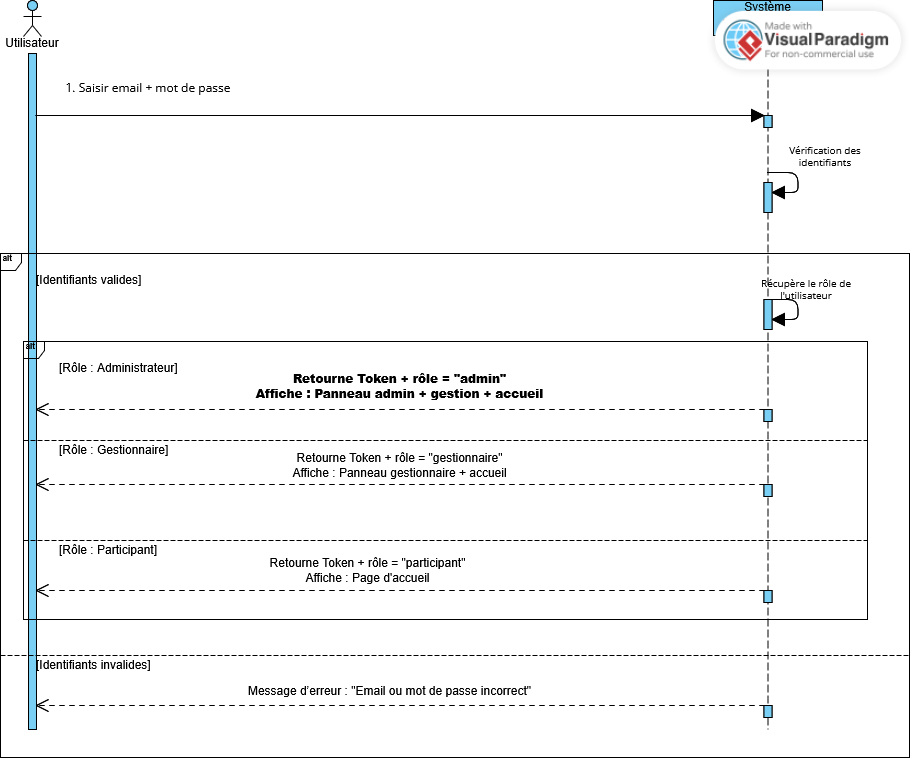
\includegraphics[width=1\linewidth]{projet/images/diagramme de sequance/diagrame de sequance s'athentifier.png}
    \caption{Diagramme de séquence « Authentification »}
    \label{fig:diagramme1}
\end{figure}

\begin{figure}[H]
    \centering
    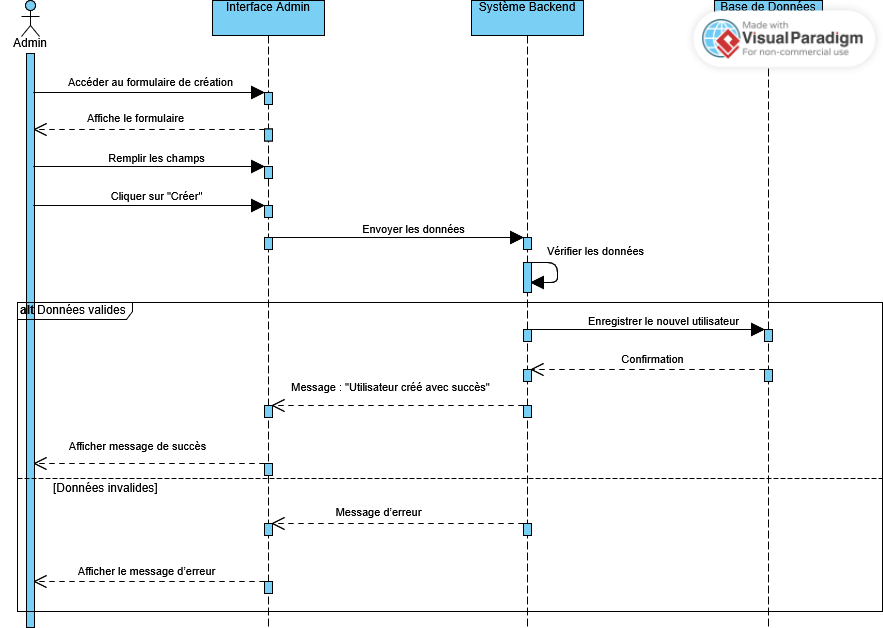
\includegraphics[width=1\linewidth]{projet/images/diagramme de sequance/cree utilisateur admin sequance diagram.png}
    \caption{Diagramme de séquence système Créer un utilisateur}
    \label{fig:diagramme2}
\end{figure}

\begin{figure}[H]
    \centering
    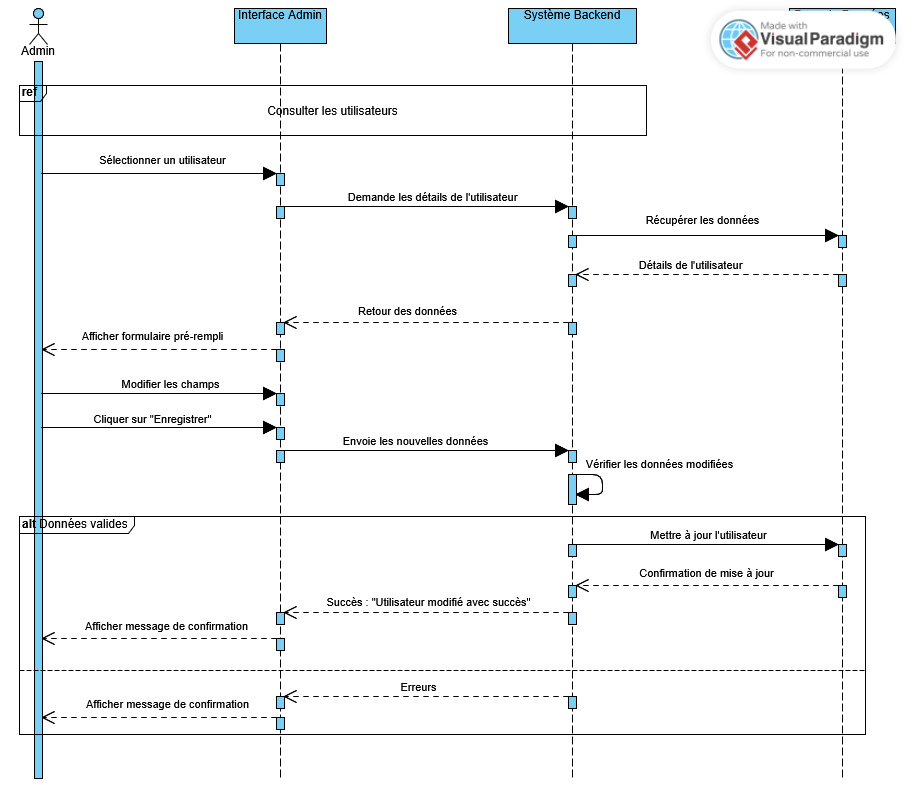
\includegraphics[width=1\linewidth]{projet/images/diagramme de sequance/modifier utlisateur admin sequance diagram.png}
    \caption{Diagramme de séquence système Modifier un utilisateur}
    \label{fig:diagramme3}
\end{figure}

\begin{figure}[H]
    \centering
    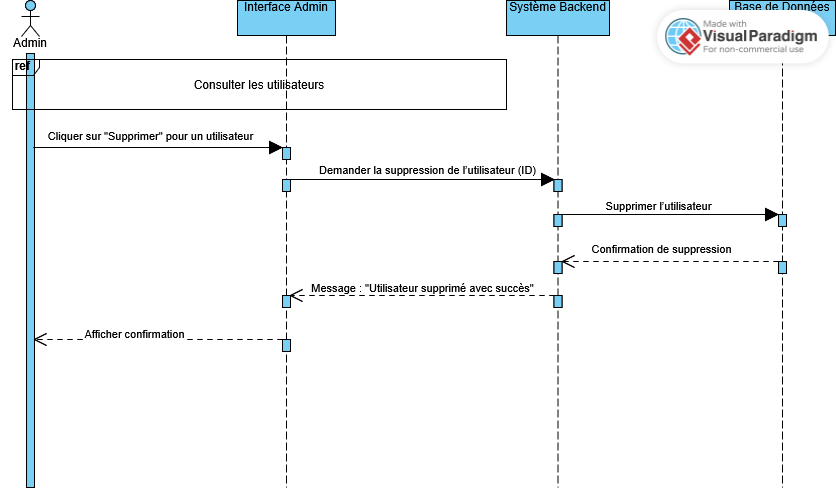
\includegraphics[width=1\linewidth]{projet/images/diagramme de sequance/supprimer utilisateur admin sequance diagram.png}
    \caption{Diagramme de séquence système Supprimer un utilisateur}
    \label{fig:diagramme4}
\end{figure}

\begin{figure}[H]
    \centering
    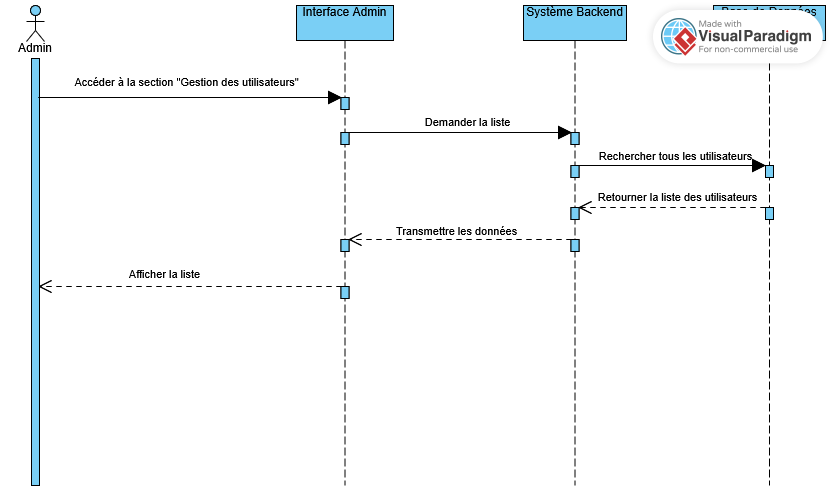
\includegraphics[width=1\linewidth]{projet/images/diagramme de sequance/consulter les utilisateurs admin sequnace diagram(1).png}
    \caption{Diagramme de séquence système Consulter un utilisateur}
    \label{fig:diagramme5}
\end{figure}

\textbf{Diagramme de classe (à compléter)}

\subsubsection{Réalisation}
Cette interface représente le formulaire d'inscription dédié à l'utilisateur et gestionnaire, comprenant les champs nom mail mot de passe.

\begin{figure}[H]
    \centering
    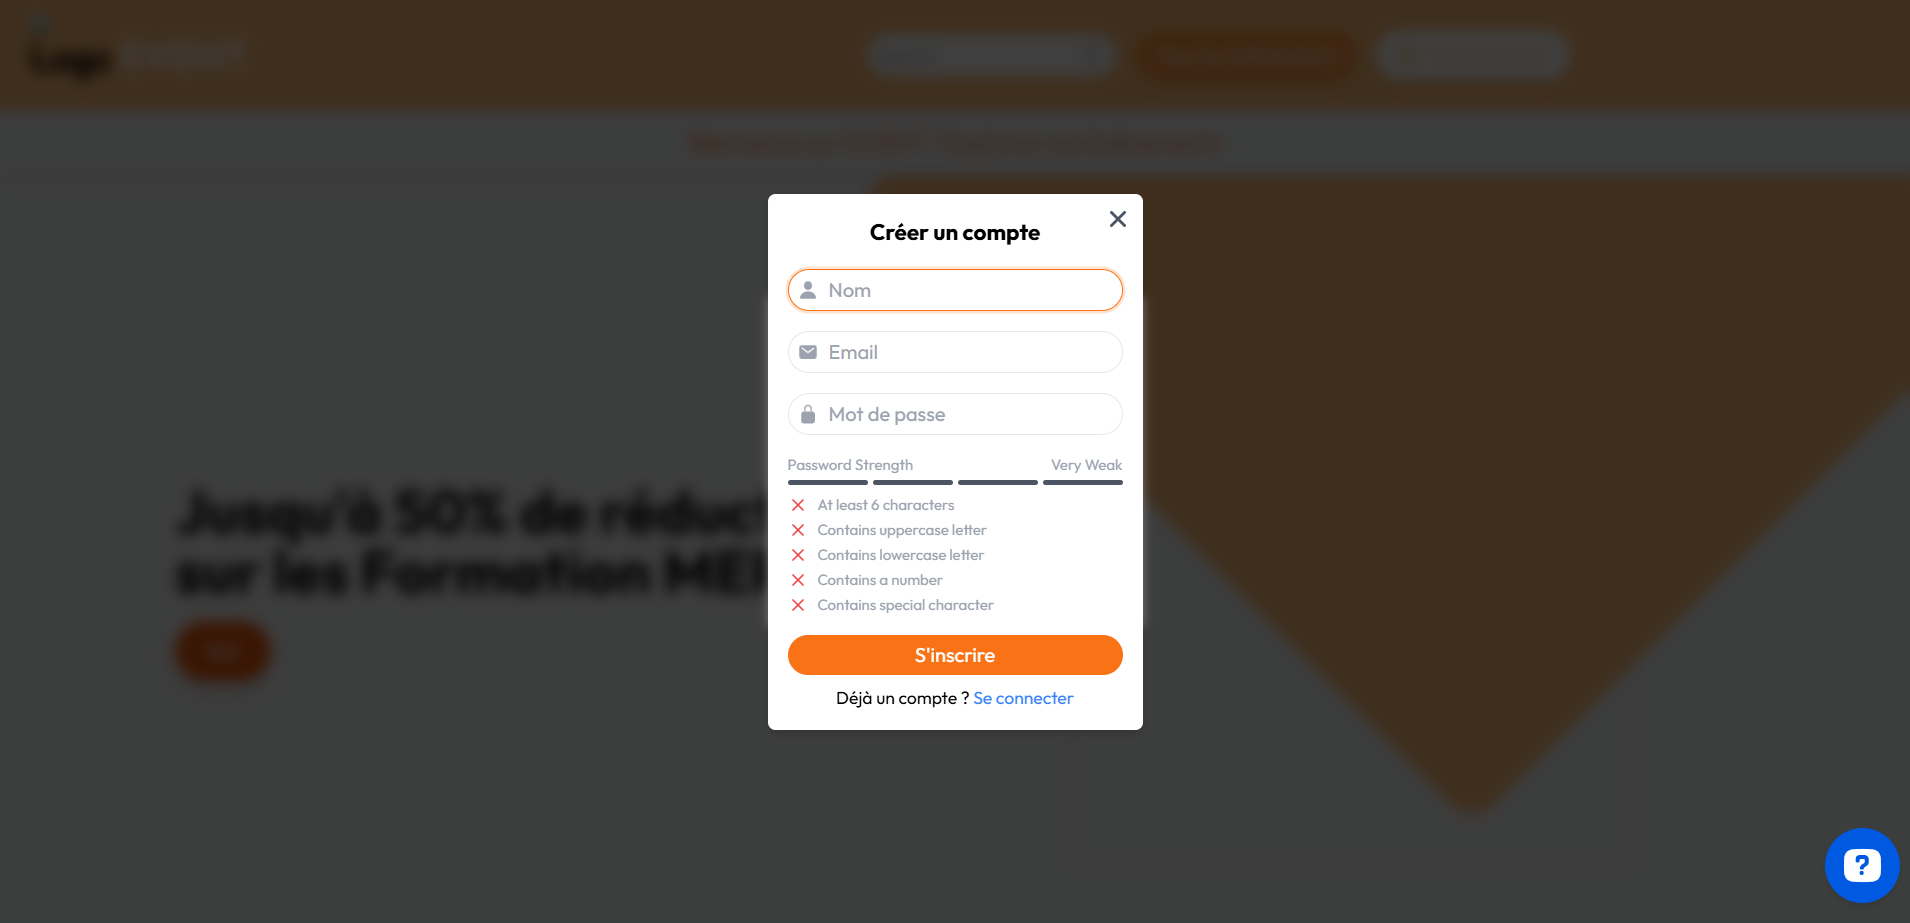
\includegraphics[width=1\linewidth]{projet/images/diagramme de sequance/images/registration.png}
    \caption{Interface graphique de creation compte}
    \label{fig:interface1}
\end{figure}

\begin{figure}[H]
    \centering
    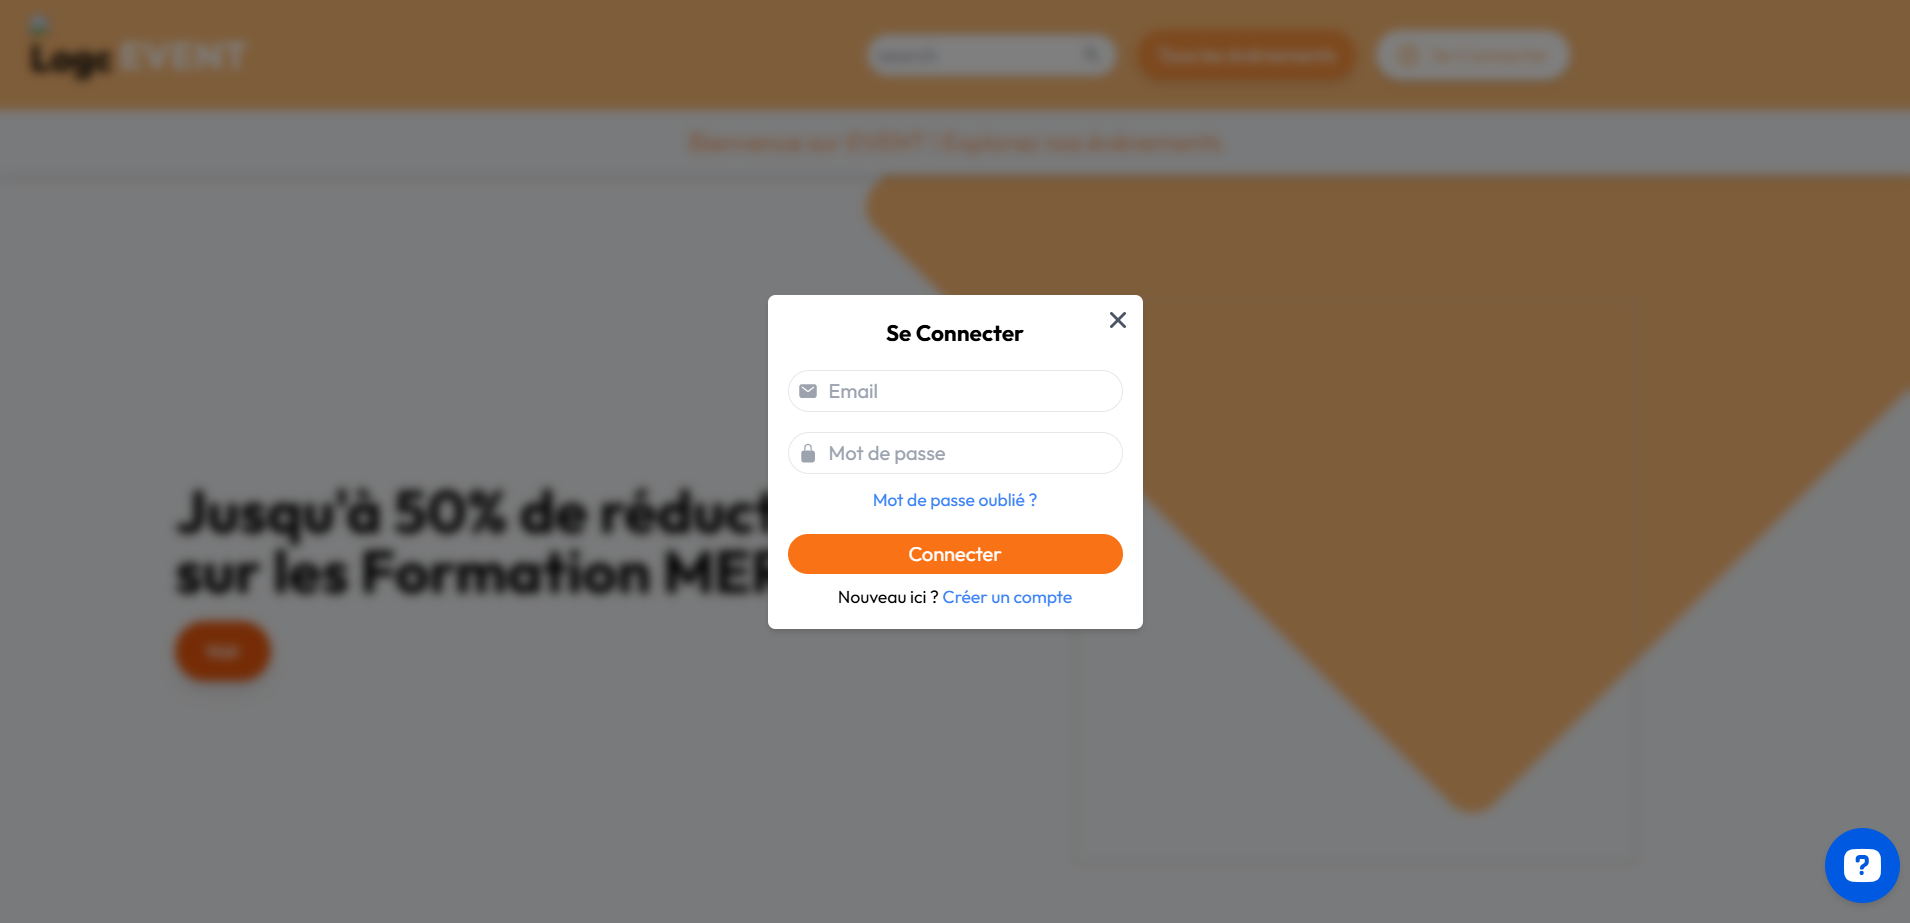
\includegraphics[width=1\linewidth]{projet/images/diagramme de sequance/images/login.png}
    \caption{Interface graphique d'authentification}
    \label{fig:interface2}
\end{figure}

Cette interface représente la page d'accueil de l'administrateur. Elle s'affiche une fois la gestion des utilisateurs.

\begin{figure}[H]
    \centering
    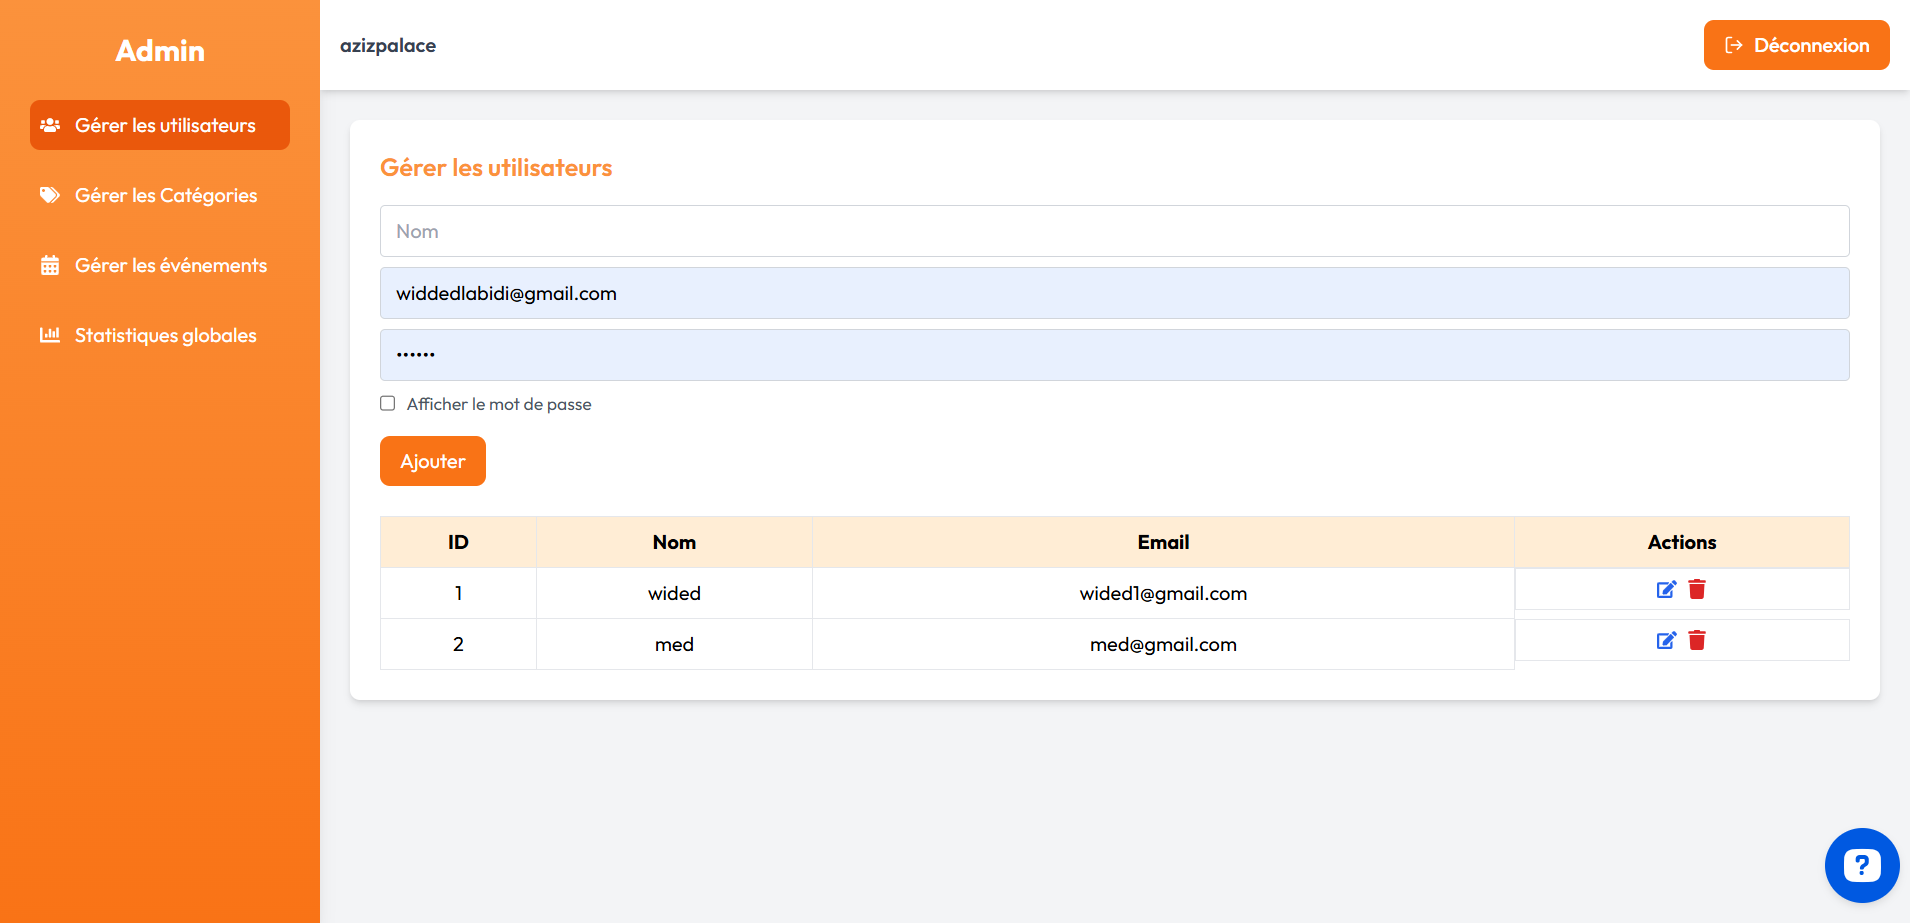
\includegraphics[width=1\linewidth]{projet/images/diagramme de sequance/images/gestion d'utilisateur.png}
    \caption{Interface graphique de gérer les utilisateurs}
    \label{fig:interface3}
\end{figure}